\appendix
\chapter{Appendix}

\section{\texorpdfstring{A brief note on the tree $H_{C,1}$}{A brief note on the tree HC1}}
\label{appx:x_plus_1_variant}
A special case of Collatz trees is the graph $H_{C,1}$ -- the $x+1$ variant of $H_C$. In this case, any sequence of successive nodes along the path from $v_n$ down to $v_1$ is strictly monotonically increasing. If we run reverse to the edge direction (towards the root), then of course the node sequence is strictly monotonically decreasing. Figure~\ref{fig:hc1} shows a portion of the graph $H_{C,1}$ starting at its root.

\begin{figure}[H]
	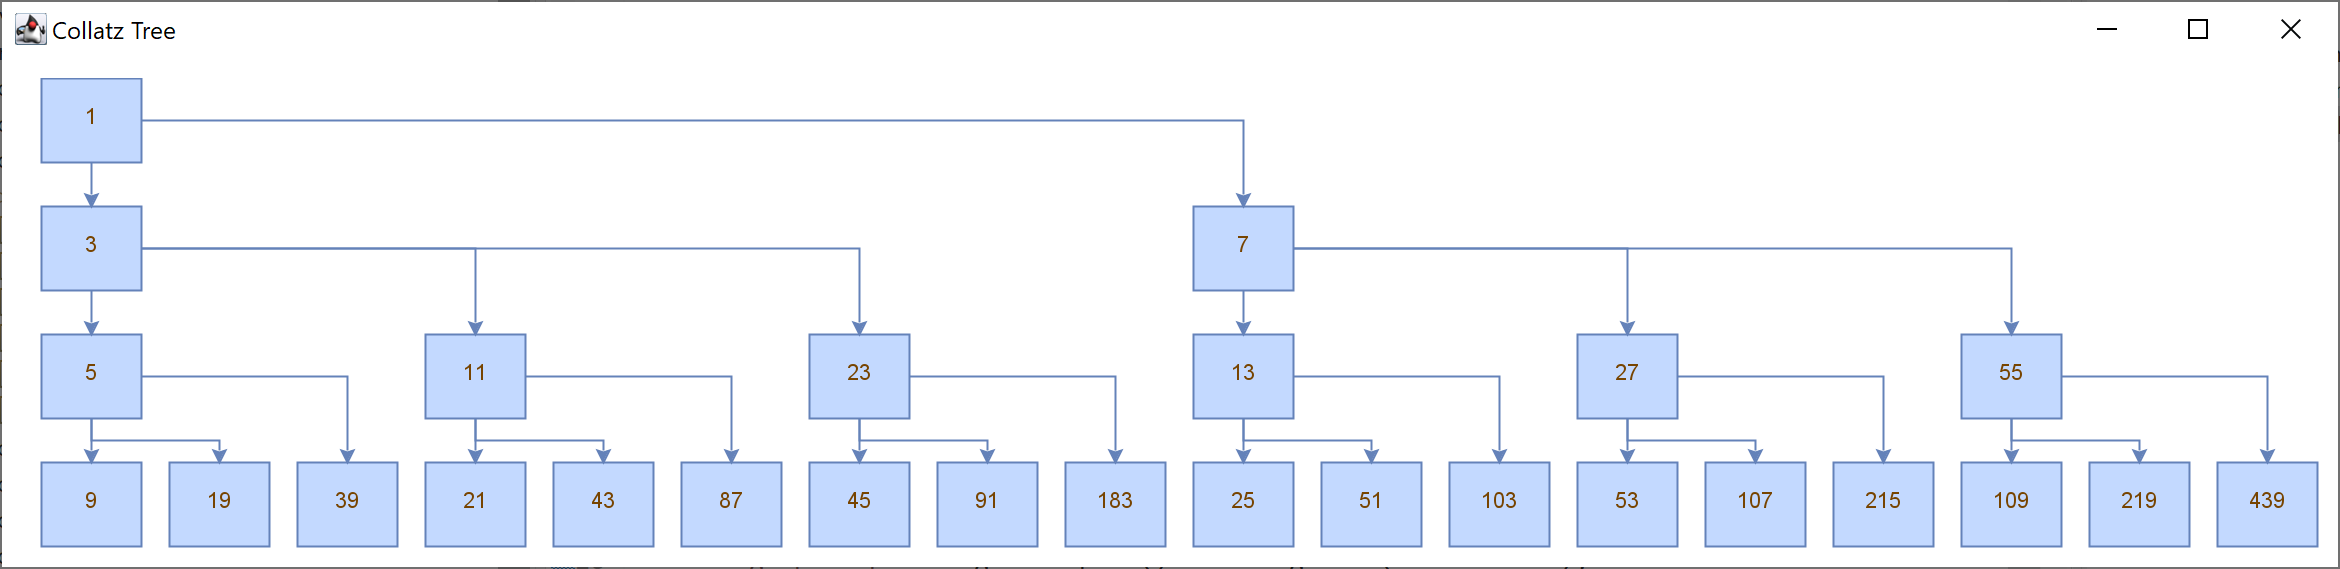
\includegraphics[width=1.00\textwidth]{figures/h_c1.png}
	\caption{Section of the graph $H_{C,1}$ starting at its root (without branches that reflect a subsequence containing the trivial cycle)}
	\label{fig:hc1}
\end{figure}

\section{\texorpdfstring{Algorithm for pruning binary trees $T_{\ge j}$}{Algorithm for pruning binary trees Tj}}
\label{appx:pruning}
Binary trees as introduced in chapter~\ref{ch:binary_tree} inspired by Kleinnijenhuis~\cite{Ref_Kleinnijenhuis_2020a}, \cite{Ref_Kleinnijenhuis_2020b} can iteratively be pruned (the way Kleinnijenhuis originally invented it). Listing~\ref{lst:pruning} implements this pruning algorithm.

\begin{listing}[H]
	\begin{minted}[bgcolor=bg, linenos, framesep=2mm, mathescape, breaklines, tabsize=2]{python}
def shrinkRoot(self):
	self.root = self.root.successors[0]
	self.root.predecessor = None

def prune(self):
	self.shrinkRoot()
	new_prunables = []
	for node in self.prunable_nodes:
		if node.predecessor is not None:
			if len(node.successors) > 1 and len(node.predecessor.successors) > 1:
				node.predecessor.successors[1].successors.append(node.successors[1])
				node.predecessor.successors[1].successors.reverse()
				node.successors[1].predecessor = node.predecessor.successors[1]
				node.successors[1].prunable = True
				new_prunables.append(node.successors[1])
			node.predecessor.successors.remove(node)
			node.predecessor = None
			self.labels.remove(node.label)
	self.prunable_nodes = new_prunables
	return self
	\end{minted}
	\caption{Python function for pruning a binary tree $T_{\ge j}$ \cite{Ref_Sultanow_Github}}
	\label{lst:pruning}
\end{listing}

Listing~\ref{lst:pruning} is only intended to illustrate the pruning algorithm in a simplifying manner. To run pruning on trees with arbitary large numbers, we refer to the professional Python API by Koch \cite{Ref_Koch_Github}.

\section{\texorpdfstring{The sum of reciprocated vertices depending only on $v_1$}{Sum of reciprocated vertices depending only on v1}}
\label{appx:sum_reciprocal_vertices}
One condition deduced from theorem~\ref{theo:1} is the product condition~\ref{eq:condition_max}, which specifies the validity of the cycle-alpha's upper limit. This condition requires the sum $\nicefrac{1}{kv_1}+\nicefrac{1}{kv_2}+\nicefrac{1}{kv_3}+\ldots$ to be limited. In order to formulate this sum independently from the successive vertices $v_2,v_3,\ldots$, we substitute these as follows:

\begin{flalign}
v_1&=v_1\notag\\
v_2&=\frac{kv_1+1}{2^{\alpha_1}}\notag\\
v_3&=\frac{k^2v_1+k+2^{\alpha_1}}{2^{\alpha_1+\alpha_2}}\notag\\
v_4&=\frac{k^3v_1+k^2+k\cdot2^{\alpha_1}+2^{\alpha_1+\alpha_2}}{2^{\alpha_1+\alpha_2+\alpha_3}}\label{eq:sum_v_4}\\
\vdots\notag\\
v_{n+1}&=\frac{k^nv_1+\sum_{j=1}^{n}k^{j-1}2^{\alpha_1+\ldots+\alpha_n-\sum_{l>n-j}\alpha_l}}{2^{\alpha_1+\ldots+\alpha_n}}\label{eq:sum_v_n_plus_1}
\end{flalign}

The sum of the reciprocated vertices can be expressed as a term that depends from $v_1$ and from the number of contracted edges, id est the number of dvisions by two, between two successive vertices $\alpha_1,\alpha_2,\alpha_3,\ldots$: 
\begin{equation*}
\sum_{i=1}^{n+1}\frac{1}{kv_i}=\frac{1}{k}\left(\frac{1}{v_1}+\sum_{i=1}^{n}\frac{1}{v_{i+1}}\right)=\frac{1}{k}\left(\frac{1}{v_1}+\sum_{i=1}^{n}\frac{2^{\alpha_1+\ldots+\alpha_i}}{k^iv_1+\sum_{j=1}^{i}k^{j-1}2^{\alpha_1+\ldots+\alpha_n-\sum_{l>i-j}\alpha_l}}\right)
\end{equation*}

\section{\texorpdfstring{The product of reciprocated vertices incremented by one}{The product of reciprocated vertices incremented by one}}
\label{appx:product_formula_depending_v1}
In a similar way to deduce the sum of reciprocated vertices depending only on $v_1$ as performed in \ref{appx:sum_reciprocal_vertices}, we evolve the product formula depending only on $v_1$:
\begin{flalign}
\prod_{i=1}^{n+1}\left(1+\frac{1}{kv_i}\right)&=1+\frac{2^{\alpha_1+\ldots+\alpha_n}+k\cdot2^{\alpha_1+\ldots+\alpha_{n-1}}+\ldots+k^{n-1}\cdot2^{\alpha_1}+k^n}{k^{n+1}v_1}\label{eq:prod_sum_v_n_plus_1}\\
&=1+\frac{2^{\alpha_1+\ldots+\alpha_n}+k\cdot\sum_{j=1}^{i}k^{j-1}2^{\alpha_1+\ldots+\alpha_n-\sum_{l>i-j}\alpha_l}}{k^{n+1}v_1}\label{eq:prod_sum_v_n_plus_1_inserted}\\
&=1+\frac{2^{\alpha_1+\ldots+\alpha_n}+k\cdot\left(v_{n+1}\cdot2^{\alpha_1+\ldots+\alpha_n}-k^nv_1\right)}{k^{n+1}v_1}\notag\\
&=\frac{2^{\alpha_1+\ldots+\alpha_n}\left(1+kv_{n+1}\right)}{k^{n+1}v_1}\label{eq:prod_sum_v_n_plus_1_simplified}
\end{flalign}
We inserted the sum used in equation~\ref{eq:sum_v_n_plus_1} into the above-given equation~\ref{eq:prod_sum_v_n_plus_1} and then obtained equation~\ref{eq:prod_sum_v_n_plus_1_inserted}. Let us divide this product by the last factor and consider the product in the condition for cycle-alpha's upper limit, which iterates to $n$ instead of $n+1$:

\begin{equation}
\label{eq:prod_sum_v_n_simplified}
\prod_{i=1}^{n}\left(1+\frac{1}{kv_i}\right)=\frac{\prod_{i=1}^{n+1}\left(1+\frac{1}{kv_i}\right)}{\frac{kv_{n+1}+1}{kv_{n+1}}}=\frac{2^{\alpha_1+\ldots+\alpha_n}\cancel{\left(1+kv_{n+1}\right)}kv_{n+1}}{k^{n+1}v_1\cancel{\left(kv_{n+1}+1\right)}}=\frac{2^{\alpha_1+\ldots+\alpha_n}v_{n+1}}{k^nv_1}
\end{equation}

The above-shown equation~\ref{eq:prod_sum_v_n_simplified} becomes simplified, when we replaced the numerator by equation~\ref{eq:prod_sum_v_n_plus_1_simplified}. The question which sequence maximizes its last member $v_{n+1}$ ties into the question: Which sequence maximizes the product? The product formula~\ref{eq:prod_sum_v_n_simplified} does not depend from all vertices $v_1,v_2,\ldots,v_n$, it depends only from $2^\alpha=2^{\alpha_1+\ldots+\alpha_n}$, from the first vertex $v_1$ and the final one $v_{n+1}$.

\section{Engel expansions maximize the node $v_{n+1}$}
A sequence $v_{n+1},v_n,\ldots,v_2,v_1$ describing a path in $H_{C,3}$ from $v_{n+1}$ down to $v_1$ allows at most one division by $2$ between two successive nodes. Dividing only once between two successive nodes, maximizes the $v_{n+1}$, but it is not obvious that this maximizes the product contained in condition~\ref{eq:condition_max}. Such a sequence forms the following ascending continued fraction (for the classical case $b=2,k=3$ see \cite[p.~11]{Ref_Laarhoven}):

\begin{equation}
	\label{eq:asc_continued_fraction}
	v_{n+1}=\cfrac{k\cfrac{k\cfrac{k\cfrac{kv_1+1}{b}+1}{b}+1}{b}+1}{b}\dotsb
	=\frac{k^nv_1+\sum_{i=0}^{n-1}k^ib^{n-1-i}}{b^n}
	=\frac{k^nv_1}{b^n}+\frac{k^n-b^n}{(k-b)b^n}
\end{equation}

\par\medskip
The sum of the products of the powers of $k$ and $b$, contained in equation \ref{eq:asc_continued_fraction}, can be simplified by converting this sum into the form $(k-b)
(b^{n-1}+kb^{n-2}+k^2b^{n-3}+\ldots+k^{n-3}b^2+k^{n-2}b+k^{n-1})=k^n-b^n$ as follows:
\begin{flalign*}
k^n-b^n=k^n\left(1-\frac{b^n}{k^n}\right)&=k^n\left(1-\frac{b}{k}\right)\left(1+\frac{b}{k}+\frac{b^2}{k^2}+\ldots+\frac{b^{n-3}}{k^{n-3}}+\frac{b^{n-2}}{k^{n-2}}+\frac{b^{n-1}}{k^{n-1}}\right)=\left(1-\frac{b}{k}\right)\sum_{i=0}^{n-1}k^n\left(\frac{b}{k}\right)^i\\
&=k\cdot\left(1-\frac{b}{k}\right)\cdot k^{n-1}\cdot\left(\frac{b^{n-1}}{k^{n-1}}+\frac{b^{n-2}}{k^{n-2}}+\frac{b^{n-3}}{k^{n-3}}+\ldots+\frac{b^2}{k^2}+\frac{b}{k}+1\right)\\
&=(k-b)
(b^{n-1}+kb^{n-2}+k^2b^{n-3}+\ldots+k^{n-3}b^2+k^{n-2}b+k^{n-1})
\end{flalign*}

\begin{example}
	A concrete example (where $b=2$ and $k=3$) for such a sequence is $v_1=31$, $v_2=47$, $v_3=71$, $v_4=107$, $v_5=161$. And, to follow that example, we can calculate the label of the vertex $v_5$ in a straightforward way:
	\[
	v_5=v_{n+1}=\frac{3^4(31+1)-2^4}{2^4}=161
	\]
	Besides, by choosing a vertex $v_1=2^{n+1}-1$, we are able to infinitely generate sequences each forming an ascending continued fraction. As per equation~\ref{eq:asc_continued_fraction} the last member in this sequence is the odd labeled vertex $v_{n+1}=3^n\cdot2-1$.
\end{example}

\begin{remark}
	Ascending variants of a continued fraction, such as used in equation~\ref{eq:asc_continued_fraction}, shall not be confused with continued fractions as treated for example in \cite{Ref_Moore}, \cite{Ref_Hensley}, \cite{Ref_Borwe_etal}. These ascending continued fractions correspond to the so-called "Engel Expansions" \cite{Ref_Kraaikamp_Wu}.
\end{remark}

\par\noindent
As illustrated below, we can formulate the ascending continued fractions in a generalized fashion, whereas the analogy to \ref{eq:asc_continued_fraction} is given by $b_1=b_2=b_3=b_4=b$ and $a_1=k^0$, $a_2=k^1$, $a_3=k^2$ and $a_4=k^3+k^4v_1$:
\[
\cfrac{a_1+\cfrac{a_2+\cfrac{a_3+\cfrac{a_4}{b_4}}{b_3}}{b_2}}{b_1}\dotsb=\frac{a_1}{b_1}+\frac{a_2}{b_1b_2}+\frac{a_3}{b_1b_2b_3}+\frac{a_4}{b_1b_2b_3b_4}+\cdots
\]

\par\medskip
The generalized equation~\ref{eq:asc_continued_fraction} may be used to compute any of the above-named ascending continued fraction that has $a_i=k^{i-1}$, $b_i=b$ for $i\in\mathbb{N}$ and $a_n=k^{n-1}+k^nv_1$.

\section{Include more divisions by two into an Engel expansion}
\label{sec:include_divisions_engel_expansion}
For calculating the largest possible $v_{n+1}$, we considered so far Engel expansions which contain only $n$ division by two within a Collatz sequence of $n+1$ memebers. In the following we include $m$ additional divisions by two and thus a total of $m+n$ divisions. We look at two corner cases:
\begin{itemize}
	\item the one where we do the additional $m$ divisions by $2$ at the end and
	\item the one where we do these additional divisions at the very beginning.
\end{itemize}

\par\noindent
\textbf{The first case} is our starting point to examine how the swapping a division by two affects the node $v_{n+1}$. For this, let us compare the Engel expansion where we devide by $2^m$ afterwards with one where we divide by $2$ in the penultimate step and by $2^{m-1}$ in last step. One can immediately recognize the following inequality with a mere look:
\[
\cfrac{1+\cfrac{3+\cfrac{3^2+\cfrac{3^3+3^4v_1}{2}}{2}}{2}}{2\cdot2^m}
<
\cfrac{1+\cfrac{3+\cfrac{3^2+\cfrac{3^3+3^4v_1}{2}}{2}}{2\cdot\textcolor{red}{\mathbf{2}}}}{2\cdot2^{m-1}}
\]

To put it simply, in the expansion on the right side of the above-shown inequality we perform one division by two a little bit earlier as we do it in the expansion on the left side of the expansion. Almost all summands of both expansions cancel out each other:

\[
\frac{1}{2\cdot2^m}+\cancel{\frac{3}{2^2\cdot2^m}+\frac{3^2}{2^3\cdot2^m}+\frac{3^3+3^4v_1}{2^4\cdot2^m}}
<
\frac{1}{2\cdot2^{m-1}}+\cancel{\frac{3}{2^2\cdot\textcolor{red}{\mathbf{2}}\cdot2^{m-1}}+\frac{3^2}{2^3\cdot\textcolor{red}{\mathbf{2}}\cdot2^{m-1}}\frac{3^3+3^4v_1}{2^4\cdot\textcolor{red}{\mathbf{2}}\cdot2^{m-1}}}
\]

\par\bigskip\noindent
\textbf{The second case} deals with Engel expansions where we perform that additional $m$ divisions by two as early as possible. The resulting value decreases, when we make a division by two later:
\[
\cfrac{1+\cfrac{3+\cfrac{3^2+\cfrac{3^3+3^4v_1}{2\cdot2^{m-1}}}{2\cdot\textcolor{red}{\mathbf{2}}}}{2}}{2}
<
\cfrac{1+\cfrac{3+\cfrac{3^2+\cfrac{3^3+3^4v_1}{2\cdot2^m}}{2}}{2}}{2}
\]

Also here almost all summands of both Engel expansions, they cancel each other out:

\[
\cancel{\frac{1}{2}+\frac{3}{2^2}}+\frac{3^2}{2^3\cdot\textcolor{red}{\mathbf{2}}}+\cancel{\frac{3^3+3^4v_1}{2^4\cdot\textcolor{red}{\mathbf{2}}\cdot2^{m-1}}}
<
\cancel{\frac{1}{2}+\frac{3}{2^2}}+\frac{3^2}{2^3}+\cancel{\frac{3^3+3^4v_1}{2^4\cdot2^m}}
\]

\par\medskip
While the first case minimizes the value of the node $v_{n+1}$, the second case maximizes it. The difference between the maximum and the minimum is given by the following equation:

\begin{flalign*}
	&\frac{3^{n-1}\left(\frac{3v_1+1}{2\cdot2^m}+1\right)-2^{n-1}}{2^{n-1}}-\frac{3^n\left(v_1+1\right)-2^n}{2^{n+m}}\\
	=&\frac{3^{n-1}\cdot\left(3v_1+1+2^{m+1}\right)-2^{n-1}\cdot2^{m+1}-3^n\left(v_1+1\right)+2^n}{2^{m+1}\cdot2^{n-1}}\\
	=&\frac{3^{n-1}+3^{n-1}\cdot2^{m+1}-2^{n+m}-3^n+2^n}{2^{n+m}}=\frac{3^{n-1}-3\cdot3^{n-1}+3^{n-1}\cdot2^{m+1}-2^{n+m}+2^n}{2^{n+m}}\\
	=&\frac{-2\cdot3^{n-1}+3^{n-1}\cdot2^{m+1}-2^{n+m}+2^n}{2^{n+m}}=\frac{\left(2\cdot3^{n-1}-2^n\right)\left(2^m-1\right)}{2^n\cdot2^m}\\
	=&\left(\frac{3^{n-1}}{2^{n-1}}-1\right)\left(1-\frac{1}{2^m}\right)
\end{flalign*}

This has the consequence that for a given sequence consisting of $n+1$ members, between which a total of $n+m$ divisions have taken place, the permutation of these divisions has a very limited effect on the node $v_{n+1}$ as described by theorem~\ref{theo:permutation}.

\par\medskip
\begin{theorem}
	\label{theo:permutation}
	Let $v_{n+1},v_n,\ldots,v_2,v_1$ be a sequence in which a total of $n+m$ divisions took place (a path in which a total of $n+m$ edges has been contracted). No matter how these divisions are permuted, i.e. performed sooner or later, the node $v_{n+1}$ can differ at most by the following product:
	\[
	\left(\frac{3^{n-1}}{2^{n-1}}-1\right)\left(1-\frac{1}{2^m}\right)
	\]
\end{theorem}

\section{The product in the condition for alpha's upper limit}
Let us take a closer look at the product contained in condition~\ref{eq:condition_max} for the case $k=3$ and use the ascending continued fractions for examining this product. The exciting question is, does this product have a limit value even in the case where we only contract a single edge between successive nodes? Setting accordingly the sequence, which maximizes $v_{n+1}$, into the product expressed by condition~\ref{eq:condition_max}, we obtain a product that is limited, or to be more specific, which in the worst case $v_1=1$ converges (for $n$ to infinity) towards $2$:
\begin{equation}
	\label{eq:product_simplification_k3}
	\prod_{i=1}^{n}\left(1+\frac{1}{3v_{i}}\right)
	=\prod_{i=1}^{n}\left(1+\frac{1}{3\frac{3^{i-1}(v_1+1)-2^{i-1}}{2^{i-1}}}\right)
	=\prod_{i=1}^{n}\frac{3^i(v_1+1)-2^i}{3^i(v_1+1)-3*2^{i-1}}
	=\frac{1}{v_1}-\frac{1}{v_1}\left(\frac{2}{3}\right)^n+1
\end{equation}

The above-illustrated last forming step, simplifies this product significantly into an expression waiving a product formulation. A detailed breakdown including all intermediate steps of this simplification is shown in the appendix~\ref{appx:product_simplification_k3}. The correctness of this simplification can be proven inductively too, which we detail in appendix~\ref{appx:proof_product_simplification_k3}. The most important and the most interesting aspect of this result is, that the above simplified term cannot exceed the value $2$, whatever you choose to insert into $n$ or into $v_1$:
\[
\frac{1}{v_1}-\frac{1}{v_1}\left(\frac{2}{3}\right)^{n+1}+1<2
\]

Since, as shown above, the product cannot exceed the value $2$, the logarithmic product expression in the condition~\ref{eq:condition_max} cannot exceed the value one and this condition becomes a consistently true statement:
\[
n\log_23-\lfloor n\log_23\rfloor<2-1
\]

Thus, for $k=3$ the condition~\ref{eq:condition_max} for alphas's upper limit is met for all sequences that maximize $v_{n+1}$.

\section{Include additional divisions into the product}
How does the product, contained in condition~\ref{eq:condition_max}, look like if we include the additional $m$ divisions into the Engel expansion as per section~\ref{sec:include_divisions_engel_expansion}? To answer this question, we consider the sequence $v_{n+1},v_n,v_{n-1},\ldots,v_2,v_1$ and we set $v_2=\frac{3v_1+1}{2\cdot2^{m}}$. Then reusing the continued fraction given by equation~\ref{eq:asc_continued_fraction}, we obtain:

{\setlength{\jot}{1.2em}
	\begin{flalign}
		\label{eq:asc_continued_fraction_m}
		v_{n+1}&=\cfrac{3\cfrac{3\cfrac{3\cfrac{3v_1+1}{2\cdot2^m}+1}{2}+1}{2}+1}{2}\dotsb
		=\cfrac{3\cfrac{3\cfrac{3v_2+1}{2}+1}{2}+1}{2}\dotsb
		=\frac{3^{n-1}(v_2+1)-2^{n-1}}{2^{n-1}}\\
		\notag
		&=\frac{3^{n-1}(\frac{3v_1+1}{2\cdot2^{m}}+1)-2^{n-1}}{2^{n-1}}=\frac{3^nv_1+3^{n-1}+3^{n-1}2^{m+1}}{2^{m+n}}-1
\end{flalign}}

\par\noindent
The product will be calculated by using equation~\ref{eq:product_simplification_k3}:
\begin{flalign}
	\label{eq:product_k3_m}
	\prod_{i=1}^{n}\left(1+\frac{1}{3v_{i}}\right)&=\left(1+\frac{1}{3v_1}\right)\cdot\prod_{i=2}^{n}\left(1+\frac{1}{3v_{i}}\right)\\
	\notag
	&=\left(1+\frac{1}{3v_1}\right)\cdot\prod_{i=1}^{n-1}\left(1+\frac{1}{3v_{i+1}}\right)=\left(1+\frac{1}{3v_1}\right)\cdot\left(\frac{1}{v_2}-\frac{1}{v_2}\left(\frac{2}{3}\right)^{n-1}+1\right)
\end{flalign}

\par\noindent
Finally substituting $v_2=\frac{3v_1+1}{2\cdot2^{m}}$ into equation~\ref{eq:product_k3_m} leads to the simplified formula of the product:
\begin{equation}
	\label{eq:product_simplification_k3_m}
	\prod_{i=1}^{n}\left(1+\frac{1}{3v_{i}}\right)=\left(1+\frac{1}{3v_1}\right)\cdot\frac{1-\left(\frac{2}{3}\right)^{n-1}+v_2}{v_2}=\frac{1+2^{m+1}}{3v_1}-\frac{2^m}{v_1}\left(\frac{2}{3}\right)^n+1
\end{equation}

\begin{example}
	An example provides the sequence $v_1=661$, $v_2=31$, $v_3=47$, $v_4=71$, $v_5=107$. When we input $v_1=661$ with $m=5$ and $n=4$ into equation~\ref{eq:asc_continued_fraction_m} we retrieve the label of the vertex $v_5$:
	\[
	v_5=v_{n+1}=\frac{3^4\cdot661+3^3+3^3\cdot2^6}{2^9}-1=107
	\]
	In this sequence five $(m=5)$ additional divisions by two took place in the first step using $v_1$:
	\[
	\frac{3\cdot661-1}{2\cdot2^5}=v_2=31
	\]
	Let us now verify the formula for the product by taking this particular example. To this end we input $v_1=661$ together with $m=5$ and $n=4$ into equation~\ref{eq:product_simplification_k3_m}:
	\[
	\left(1+\frac{1}{3\cdot661}\right)\left(1+\frac{1}{3\cdot31}\right)\left(1+\frac{1}{3\cdot47}\right)\left(1+\frac{1}{3\cdot71}\right)=\frac{1+2^{6}}{3\cdot661}-\frac{2^5}{661}\left(\frac{2}{3}\right)^4+1=1.023215853
	\]
\end{example}

\section{Condition for a limited growth of the Engel expansion}
\label{sec:condition_limited_growth}
Let us look now into the question of what condition must be met to prevent a greater growth than a decline in Collatz sequences. Specifically we consider an Engel expansion comprising $n+1$ sequence members that include $m$ additional divisions by two at the beginning. The last member $v_{n+1}$ in such a sequence can be calulated by formula~\ref{eq:asc_continued_fraction_m}. In order to restrict the growth of this sequence, we require that the last member has to be smaller than the first one. For this we define the condition $v_{n+1}<v_1$:

\[
\frac{3^nv_1+3^{n-1}+3^{n-1}2^{m+1}}{2^{m+n}}-1<v_1
\]

By transforming this inequality, which is thoroughly described in the appendix~\ref{appx:condition_limited_growth} step by step, we obtain the condition:

\begin{equation}
	\label{eq:condition_limited_growth}
	\frac{3^{n-1}\left(2^{m+1}-2\right)}{2^{m+n}-3^n}-1<v_1
\end{equation}

\section{Engel expansions maximize the product}
The question which sequence maximizes the target node $v_{n+1}$ ties into the question which sequence maximizes the product in the condition for cycle-alpha's upper limit given by equation~\ref{eq:condition_max}. The product formula that do not depend from all vertices $v_1,v_2,\ldots v_n$ has been evolved in appendix~\ref{appx:product_formula_depending_v1}. This formla depends only from $2^\alpha$, from the starting node $v_1$ and the target node $v_{n+1}$:

\[
\prod_{i=1}^{n}\left(1+\frac{1}{kv_i}\right)=\frac{2^{\alpha_1+\ldots+\alpha_n}v_{n+1}}{k^nv_1}
\]

In order to maximize this product, one needs to maximize the target node $v_{n+1}$, which exactly the Engel expansion does. Hence, for a given $v_1$, the Engel expansion is the worst case sequence maximizing the product in the condition for cycle-alpha's upper limit.
